% !TEX encoding = UTF-8 Unicode.

% Based on https://github.com/Miracle0565/BUCT-Beamer-Theme

\documentclass[
10pt,
aspectratio=43,
]{beamer}
\setbeamercovered{transparent=10}
\usetheme[
%  showheader,
%  red,
  purple,
%  gray,
%  graytitle,
  colorblocks,
%  noframetitlerule,
]{Verona}

\usepackage[T1]{fontenc}
\usepackage{tikz}
\usepackage[utf8]{inputenc}
\usepackage{lipsum}
\usepackage{pgfplots}
%%%%%%%%%%%%%%%%%%%%%%%%%%%%%%%
% Mac上使用如下命令声明隶书字体, windows也有相关方式, 大家可自行修改
\providecommand{\lishu}{\CJKfamily{zhli}}
%%%%%%%%%%%%%%%%%%%%%%%%%%%%%%%
\usepackage{tikz}
\usetikzlibrary{fadings}
%
%\setbeamertemplate{sections/subsections in toc}[ball]
\usepackage{xeCJK}
\usepackage{listings}
\usepackage{caption}
\usepackage{subfigure}
\usefonttheme{professionalfonts}
\def\mathfamilydefault{\rmdefault}
\usepackage{amsmath}
\usepackage{multirow}
\usepackage{booktabs}
\usepackage{bm}
\usepackage{mathtools}
\usepackage[T1]{fontenc}
\setbeamertemplate{section in toc}{\hspace*{1em}\inserttocsectionnumber.~\inserttocsection\par}
\setbeamertemplate{subsection in toc}{\hspace*{2em}\inserttocsectionnumber.\inserttocsubsectionnumber.~\inserttocsubsection\par}
\setbeamerfont{subsection in toc}{size=\small}
\AtBeginSection[]{%
	\begin{frame}%
		\frametitle{Outline}%
		\textbf{\tableofcontents[currentsection]} %
	\end{frame}%
}

\AtBeginSubsection[]{%
	\begin{frame}%
		\frametitle{Outline}%
		\textbf{\tableofcontents[currentsection, currentsubsection]} %
	\end{frame}%
}

\pgfplotsset{
    integral segments/.code={\pgfmathsetmacro\integralsegments{#1}},
    integral segments=3,
    integral/.style args={#1:#2}{
        ybar interval,
        domain=#1+((#2-#1)/\integralsegments)/2:#2+((#2-#1)/\integralsegments)/2,
        samples=\integralsegments+1,
        x filter/.code=\pgfmathparse{\pgfmathresult-((#2-#1)/\integralsegments)/2}
    }
}


\title{高等数学C}
%\subtitle{A Simple while elegant template}
\author[P.Yu]{余沛}
\mail{peiy\_gzgs@qq.com}
\institute[Guangzhou College of Technology and Business]{Guangzhou College of Technology and Business \\
  广州工商学院}
\date{\today}
\titlegraphic[width=4cm]{logo.png}{}




%%%%%%%%%%%%%%%%%%%%%%%%%%%%%%%%
% ----------- 标题页 ------------
%%%%%%%%%%%%%%%%%%%%%%%%%%%%%%%%



\begin{document}

\maketitle

%%% define code
\defverbatim[colored]\lstI{
	\begin{lstlisting}[language=C++,basicstyle=\ttfamily,keywordstyle=\color{red}]
	int main() {
	// Define variables at the beginning
	// of the block, as in C:
	CStash intStash, stringStash;
	int i;
	char* cp;
	ifstream in;
	string line;
	[...]
	\end{lstlisting}
}
%%%%%%%%%%%%%%%%%%%%%%%%%%%%%%%%
% ----------- FRAME ------------
%%%%%%%%%%%%%%%%%%%%%%%%%%%%%%%%

\section{定积分的概念}
\subsection{例子}
\subsubsection{面积}
\begin{frame}
	\frametitle{面积的性质}
	\everymath{\displaystyle}
	\pause
	回顾一下面积的概念, 对于任意(可以求面积的)集合$A_1, A_2,\cdots A_n$, 面积函数 $m(\cdot)$ 为从集合到非负实数的映射, 应该至少具有以下几个性质:
	\vspace{0.5cm}
	\begin{enumerate}
		\item<1-> 单调性: 若 $A_1\subset A_2$, 那么 $m(A_1)\le m(A_2)$;
		\item<2-> 并可测性: 可求面积的集合的并可求面积, $m\left(\bigcup_{i=1}^{\infty} E_i\right) \leq \sum_{i=1}^{\infty} m\left(E_i\right)$.
	\end{enumerate}
	\vspace{1cm}
	\pause
	那么, 对于一般的集合, 怎么定义"面积映射", 或者说, "面积".
\end{frame}

\begin{frame}
	\frametitle{面积的性质}
	\everymath{\displaystyle}
	\pause
	回顾一下面积的概念, 我们知道: 对于长方形来说
	\[
		\text{面积}=\text{长}\times\text{宽}.
	\]
	\pause
	对于直角三角形, 也有:
	\[
		\text{面积}=\frac12\times\text{底}\times\text{高}.
	\]
	\pause
	Wait, 回顾并可测性:
	\begin{quote}
		可求面积的集合的并可求面积, $m\left(\bigcup_{i=1}^{\infty} E_i\right) \leq \sum_{i=1}^{\infty} m\left(E_i\right)$.
	\end{quote}
	\pause
	暂时只能得到:
	\[
		\text{面积}\le\frac12\times\text{底}\times\text{高}.
	\]
	\pause
	而且, 我们总希望用尽可能简单地定义来进行面积的定义.
\end{frame}

\begin{frame}
	\frametitle{三角形的面积计算}
	\everymath{\displaystyle}
	\begin{columns}
		\begin{column}{0.6\textwidth}
			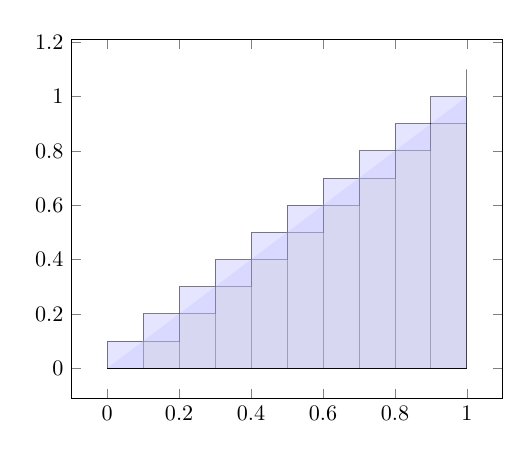
\begin{tikzpicture}[scale=0.8]
				\begin{axis}
					\addplot[const plot mark right,fill=yellow!20]
					coordinates
						{(0,0) (0.1,0.0) (0.2,0.1) (0.3,0.2)
							(0.4,0.3) (0.5,0.4) (0.6,0.5) (0.7,0.6)
							(0.8,0.7) (0.9,0.8) (1,0.9) }\closedcycle;

					\addplot[const plot,fill=blue!20,opacity=0.5]
					coordinates
						{(0,0.1) (0.1,0.2) (0.2,0.3) (0.3,0.4)
							(0.4,0.5) (0.5,0.6) (0.6,0.7) (0.7,0.8)
							(0.8,0.9) (0.9,1) (1,1.1) }\closedcycle;
					\addplot[const plot,fill=blue!20,opacity=0.5]
					coordinates
						{(0.2,0.2) (0.2,0)};
					\addplot[const plot,fill=blue!20,opacity=0.5]
					coordinates
						{(0.3,0.3) (0.3,0)};
					\addplot[const plot,fill=blue!20,opacity=0.5]
					coordinates
						{(0.4,0.4) (0.4,0)};
					\addplot[const plot,fill=blue!20,opacity=0.5]
					coordinates
						{(0.5,0.5) (0.5,0)};
					\addplot[const plot,fill=blue!20,opacity=0.5]
					coordinates
						{(0.6,0.6) (0.6,0)};
					\addplot[const plot,fill=blue!20,opacity=0.5]
					coordinates
						{(0.7,0.7) (0.7,0)};
					\addplot[const plot,fill=blue!20,opacity=0.5]
					coordinates
						{(0.8,0.8) (0.8,0)};
					\addplot[const plot,fill=blue!20,opacity=0.5]
					coordinates
						{(0.9,0.9) (0.9,0)};
					\addplot[const plot,fill=blue!20,opacity=0.5]
					coordinates
						{(0,0) (1,1)};
				\end{axis}
			\end{tikzpicture}
		\end{column}
		\begin{column}{0.5\textwidth}
			\pause
			对于高为 $1$, 底为 $1$ 的直角三角形($R$)的底进行 $n$ 次均分分块. \\\vspace{0.2cm}
			\pause 可以看到每一个分块 $\left[\frac{k-1}{n},\frac{k}{n}\right]$ 中, 高取右端点值的长方形的并($S_{\text{高}}$)可以覆盖三角形, 高取左端点值的长方形的并($S_{\text{低}}$)则可以被三角形覆盖.\\\vspace{0.2cm}
			\pause
			$$
				m(S_{\text{高}})\ge m(R)\ge m(S_{\text{低}}).
			$$
			\\\vspace{0.5cm}
			\pause
			接下来我们根据这种思维介绍: Riemann积分, Darboux积分, Riemann-Stieltjes积分的相关思想
		\end{column}
	\end{columns}
\end{frame}

\begin{frame}
	\frametitle{划分与精细化划分}
	\pause
	\begin{block}{划分, 子区间, 子区间长度}
		定义 闭区间 $[a, b]$ 的划分 $\mathrm{P}$: 是指在此区间中取一个有限的点列 $a=x_0<x_1<x_2<\ldots<x_n=b$. 每个闭区间 $\left[x_i, x_{i+1}\right]$ 叫做子区间. $\Delta x_i = x_{i+1}- x_i$ 为每个子区间的长度.
	\end{block}
	\vspace{0.2cm}
	\pause
	\begin{block}{划分的长度}
		定义 $r(P)$ 为这些子区间长度的最大值: $\displaystyle\lambda=\max_{i=1,\cdots ,n-1} \left(x_{i+1}-x_i\right)$.
	\end{block}
	\vspace{0.2cm}
	\pause
	\begin{block}{精细}
		如果划分 $\mathrm{P}'$ 是在划分$\mathrm{P}$的基础上添加一些分点和标记, 就成前者比后者更精细. (精细是一个偏序关系)
	\end{block}
	\pause
	精细化划分的例子
	\begin{align*}
		\mathrm{P}:a=x_0<x_1<x_i<\qquad \qquad x_{i+1}<\cdots<x_n=b \\
		\mathrm{P}':a=x_0<x_1<x_i<x_{i+1}<x_{i+2}<\cdots<x_{n+1}=b
	\end{align*}
\end{frame}

\begin{frame}
	\frametitle{曲边梯形的面积计算方式:Riemann积分}
	\begin{columns}
		\begin{column}{0.7\textwidth}
			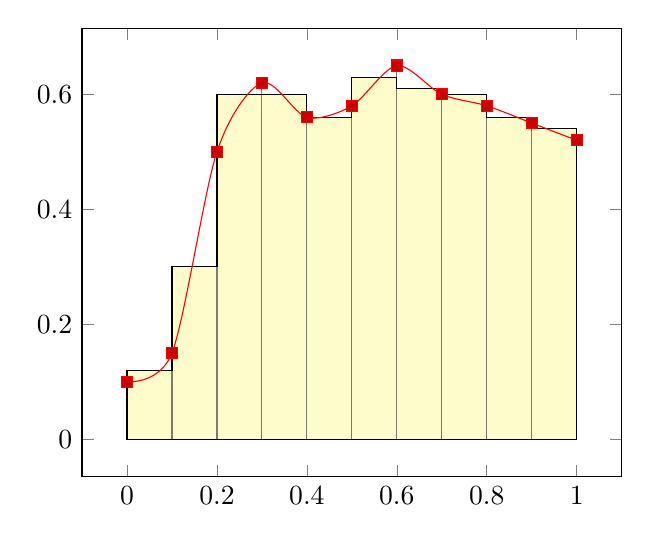
\begin{tikzpicture}[scale=1]
				\begin{axis}
					\addplot[const plot mark right,fill=yellow!20]
					coordinates
						{(0,0.07) (0.1,0.12) (0.2,0.3) (0.3,0.60)
							(0.4,0.6) (0.5,0.56) (0.6,0.63) (0.7,0.61)
							(0.8,0.6) (0.9,0.56) (1,0.54) }\closedcycle;
					\addplot+[smooth]
					coordinates
						{(0,0.1) (0.1,0.15) (0.2,0.5) (0.3,0.62)
							(0.4,0.56) (0.5,0.58) (0.6,0.65) (0.7,0.6)
							(0.8,0.58) (0.9,0.55) (1,0.52)};
					\addplot[const plot,fill=blue!20,opacity=0.5]
					coordinates
						{(0.1,0.15) (0.1,0)};
					\addplot[const plot,fill=blue!20,opacity=0.5]
					coordinates
						{(0.2,0.5) (0.2,0)};
					\addplot[const plot,fill=blue!20,opacity=0.5]
					coordinates
						{(0.3,0.62) (0.3,0)};
					\addplot[const plot,fill=blue!20,opacity=0.5]
					coordinates
						{(0.4,0.56) (0.4,0)};
					\addplot[const plot,fill=blue!20,opacity=0.5]
					coordinates
						{(0.5,0.58) (0.5,0)};
					\addplot[const plot,fill=blue!20,opacity=0.5]
					coordinates
						{(0.6,0.65) (0.6,0)};
					\addplot[const plot,fill=blue!20,opacity=0.5]
					coordinates
						{(0.7,0.6) (0.7,0)};
					\addplot[const plot,fill=blue!20,opacity=0.5]
					coordinates
						{(0.8,0.58) (0.8,0)};
					\addplot[const plot,fill=blue!20,opacity=0.5]
					coordinates
						{(0.9,0.55) (0.9,0)};
				\end{axis}
			\end{tikzpicture}
		\end{column}
		\begin{column}{0.4\textwidth}
			$\xi_k\in\left[x_{k-1},x_{k-1}+\Delta x_k\right]$为
			子区间 $\left[x_{k-1},x_{k-1}+\Delta x_k\right]$中取任意值.
		\end{column}
	\end{columns}
	$$
		S=\sum_k \Delta S_k \approx \sum_k f\left(\xi_k\right) \Delta x_k \Rightarrow S=\lim _{\lambda \rightarrow 0} \sum_k f\left(\xi_k\right) \Delta x_k.
	$$
	\pause
	这种划分的极限就是所谓的 Riemann 积分的想法.
\end{frame}


\subsection{Riemann 积分的定义}
\begin{frame}
	\frametitle{Riemann 积分的定义}
	\everymath{\displaystyle}
	\pause
	回顾求面积的方式, 我们提出Riemann 积分的定义:
	\pause
	\begin{block}{Riemann 积分的定义}
		设$f(x)$在区间$[a,b]$上有定义, $\mathrm{P}:a=x_0<x_1<x_2<\ldots<x_n=b$.
		在每段$[x_{i-1},x_i]$上 {\bf 任意}选取点$\xi_i$, 得到近似和
		$$
			\sum_{i=1}^n f(\xi_i)(x_i-x_{i-1}).
		$$
		如果对于$\mathrm{P}$的精细化
		我们就称$f(x)$在区间$[a,b]$上是 {\bf Riemann 可积}的, 并将这个极限值称为$f(x)$在$[a,b]$上的 {\bf Riemann 积分}, 记为
		\[
			\lim_{\lambda\to 0} \sum_{i=1}^n f(\xi_i)(x_i-x_{i-1}) := \int_a^b f(x)\mathrm{~d} x.
		\]
	\end{block}
	\pause
	那么, 什么情况下Riemann积分可以求出来呢?
\end{frame}

\begin{frame}
	\frametitle{Riemann积分的等价定义: Darboux积分}
	\begin{block}{}
		设$f(x)$在区间$[a,b]$上有定义, $\mathrm{P}:a=x_0<x_1<x_2<\ldots<x_n=b$.
		在每段$[x_{i-1},x_i]$上,
		$$M_i=\sup _{x \in\left[x_{i-1}, x_i\right]} f(x),\,\,m_i=\inf _{x \in\left[x_{i-1}, x_i\right]} f(x)$$
		\pause  $f(x)$在$\mathrm{P}$划分的Darboux 上下和定义为
		$$
			U_{f, P}=\sum_{i=1}^n M_i\left(x_i-x_{i-1}\right),\,\,\,\,L_{f, P}=\sum_{i=1}^n m_i\left(x_i-x_{i-1}\right)
		$$
		\pause  $f$ 的上Darboux积分指的是所有上Darboux和的下确界, $f$ 的下Darboux积分指的是所有上Darboux和的上确界:
		$$
			U_f=\inf \left\{U_{f, P}: \mathrm{P}\text{为划分}  \right\},\,\,L_f=\sup \left\{L_{f, P}: \mathrm{P}\text{为划分}\right\}.
		$$
		\pause  如果 $U_f=L_f$ 那么 $f$ 就称作Darboux可积的, 并用 $\int_a^b f(t) \mathrm{~d} t$ 表示, 记作 $f$ 在区间 $[a, b]$ 的Darboux积分.
	\end{block}
\end{frame}

\begin{frame}
	\frametitle{Darboux 积分与 Riemann积分的关系}
	\everymath{\displaystyle}
	\begin{block}{Darboux 积分与 Riemann积分的关系}
		\begin{enumerate}
			\item<1-> 对于任意划分 $\mathrm{P}$ 和任意$\xi_i\in\left[x_{i-1}, x_i\right] $ 有
				$$
					L_{f,\mathrm{P}}\le \sum_{i=1}^n f(\xi_i)(x_i-x_{i-1}) \le U_{f,\mathrm{P}}.
				$$
			\item<2-> 由 Riemann 积分中 $\xi_i$  选取的任意性, 对于连续函数, 存在选取的 $\{\xi_{l_i}\}, \{\xi_{u_i}\}$, 使得
				$$
					\sum_{i=1}^n f(\xi_{l_i})(x_i-x_{i-1})=L_{f,\mathrm{P}},\,\,\,\, \sum_{i=1}^n f(\xi_{u_i})(x_i-x_{i-1})=U_{f,\mathrm{P}}.
				$$
			\item<3-> Darboux 可积与 Riemann 可积等价.
		\end{enumerate}
	\end{block}
	\pause
	分析函数可积性: $D(x)=\begin{cases}
			1, x\in \mathbb{Q}, \\
			0, x\in \mathbb{R}/\mathbb{Q},
		\end{cases}
		\text{和}\quad R(x)=\begin{cases}
			\frac{1}{q}, x=\frac{p}{q}\in \mathbb{Q}, \\
			0, x\in \mathbb{R}/\mathbb{Q},
		\end{cases}
	$
\end{frame}

\subsubsection{定积分的极限定义}
\subsection{定义法求积分}
\section{定积分的性质}
\subsection{基本性质}

\begin{frame}
	\frametitle{定积分}
	我们已经定义
	\[
		\int_a^b f(x)\mathrm{~d}x  = \lim_{\Delta x\to 0} \sum_{i=1}^n f(\xi_i)\Delta x_i
	\]
	其中:
	\begin{itemize}
		\item<1-> $x$称为{\bf 积分变量}, $f(x)$称为{\bf 被积函数}, $f(x)\mathrm{~d}x$称为{\bf 被积表达式}
		\item<2-> $a$称为{\bf 积分下限}, $b$称为{\bf 积分上限}, $[a,b]$称为{\bf 积分区间}
	\end{itemize}
	\pause
	\begin{block}{}
		定积分的值只与被积函数$f$和积分区间$[a,b]$有关, 而与积分变量用什么字母无关.即有
		\[
			\int_a^b f(x)\mathrm{~d}x = \int_a^b f(t)\mathrm{~d}t = \int_a^b f(u)\mathrm{~d}u.
		\]
		如果$f(x)$在区间$[a,b]$上是连续函数(或者是只有有限个间断点的有界函数), 则它在$[a,b]$上是可积的.
	\end{block}
\end{frame}

\begin{frame}
	\frametitle{定积分}
	\begin{block}{}
		如果$a>b$, 我们规定
		$$
			\int_a^b f(x)\mathrm{~d} x = -\int_b^a f(x)\mathrm{~d} x,\text{ 特别地, 若 }\,\,a=b,\quad \int_a^b f(x)\mathrm{~d} x = 0 .
		$$
	\end{block}
	\begin{block}{}
		设由曲线$y=f(x)$, 直线$x=a$, $x=b$, 和$x$轴所围成的曲边梯形的面积为$S$
		\begin{itemize}
			\item 如果在$[a,b]$上$f(x)\geq 0$, 则定积分
			      $$
				      \int_a^b f(x)\mathrm{~d} x=S.
			      $$\
			\item 如果在$[a,b]$上$f(x)\leq 0$, 则定积分$$\int_a^b f(x)\mathrm{~d} x=-S.$$
		\end{itemize}
	\end{block}
\end{frame}


\begin{frame}
	\begin{block}{数乘性质}设$k$为常数, 则有
		\[
			\int_a^b kf(x)\mathrm{~d} x=k\int_a^b f(x)\mathrm{~d} x.
		\]
	\end{block}
	\pause
	\begin{block}{函数可加性}
		\[
			\int_a^b [f(x) \pm g(x)]\mathrm{~d} x = \int_a^b f(x)\mathrm{~d} x \pm \int_a^b g(x) \mathrm{~d} x.
		\]
	\end{block}
	\pause
	\begin{block}{区间可加性}
		设$a<c<b$, 则有
		\[
			\int_a^b f(x)\mathrm{~d} x = \int_a^c f(x)\mathrm{~d} x + \int_c^b f(x)\mathrm{~d} x.
		\]
	\end{block}
	\pause
	即使$c$不在$a$和$b$之间, 上述性质依然是成立的.
\end{frame}

\begin{frame}
	\begin{block}{}
		\[
			\int_a^b 1\mathrm{~d} x = \int_a^b \mathrm{~d} x= b-a.
		\]
	\end{block}
	\pause
	\begin{block}{}
		设在区间$[a,b]$上$f(x)\geq g(x)$, 则有
		\[
			\int_a^b f(x)\mathrm{~d} x \geq \int_a^b g(x)\mathrm{~d} x.
		\]
		特别地, 如果在区间$[a,b]$上$f(x)\geq 0$, 则有
		\[
			\int_a^b f(x)\mathrm{~d} x \geq 0.
		\]
	\end{block}
	\pause
	\begin{block}{}
		$$
			\left|\,\int_a^b f(x)\mathrm{~d} x\,\right| \le \int_a^b\big|f(x)\big|\mathrm{~d} x.
		$$
	\end{block}
\end{frame}

\begin{frame}
	\frametitle{比较积分大小}
	\everymath{\displaystyle}
	\begin{block}{}
		\begin{columns}
			\begin{column}{0.5\textwidth}
				\begin{enumerate}
					\item $\int_0^1 x \mathrm{~d} x$ 和 $\int_0^1 x^2 \mathrm{~d} x$;
					\item	$\int_{-\frac{\pi}{2}}^0 \sin x \mathrm{~d} x$ 和 $\int_0^{\frac{\pi}{2}} \sin x \mathrm{~d} x$;
				\end{enumerate}
			\end{column}
			\begin{column}{0.5\textwidth}
				\begin{enumerate}
					\setcounter{enumi}{2}
					\item $\int_1^2 x \mathrm{~d} x$ 和 $\int_1^2 x^2 \mathrm{~d} x$;
					\item $\int_0^{\frac{\pi}{4}} \sin x \mathrm{~d} x$ 和 $\int_0^{\frac{\pi}{4}} \cos x \mathrm{~d} x$.
				\end{enumerate}
			\end{column}
		\end{columns}
	\end{block}
	\pause
	\begin{exampleblock}{}
		\begin{columns}
			\begin{column}{0.5\textwidth}
				\begin{enumerate}
					\item<1-> $\int_0^1 x \mathrm{~d} x\ge\int_0^1 x^2 \mathrm{~d} x$;
					\item<2-> $\int_{-\frac{\pi}{2}}^0 \sin x \mathrm{~d} x\le\int_0^{\frac{\pi}{2}} \sin x \mathrm{~d} x$;
				\end{enumerate}
			\end{column}
			\begin{column}{0.5\textwidth}
				\begin{enumerate}
					\setcounter{enumi}{2}
					\item<3-> $\int_1^2 x \mathrm{~d} x\le\int_1^2 x^2 \mathrm{~d} x$;
					\item<4-> $\int_0^{\frac{\pi}{4}} \sin x \mathrm{~d} x=\int_0^{\frac{\pi}{4}} \cos x \mathrm{~d} x$.
				\end{enumerate}
			\end{column}
		\end{columns}
	\end{exampleblock}
\end{frame}

\subsection{中值定理}
\begin{frame}
	\begin{block}{积分中值定理}
		设$f(x)$在$[a,b]$上连续, 则在$[a,b]$中至少存在一点$\xi$, 使得
		\[ \int_a^b f(x)\mathrm{~d} x = f(\xi)(b-a) \]
	\end{block}
	\pause
	\begin{block}{}上述性质也是说, 存在$\xi\in[a,b]$, 使得
		\[ \frac1{b-a} \int_a^b f(x)\mathrm{~d} x = f(\xi)\]
		说明连续函数在区间$[a,b]$上的平均值是可以取到的.
	\end{block}
\end{frame}

\subsection{归纳}
\begin{frame}
	\frametitle{归纳:}
	\everymath{\displaystyle}
	\begin{enumerate}
		\item 线性性: $\int_a^b[k_1f_1(x) + k_2f_2(x)] \mathrm{d} x=\int_a^b k_1f_1(x) \mathrm{~d} x+\int_a^b k_2f_2(x) \mathrm{~d}x$;
		\item 区间可加性: $\int_a^b f(x) \mathrm{~d} x=\int_a^c f(x) \mathrm{~d} x+\int_c^b f(x) \mathrm{~d} x$;
		\item 保号性: $f(x) \geq 0, x\in[a,b]$, 则 $\int_a^b f(x) \mathrm{~d} x\geq 0$;
		\item 上下界估计: $(b-a)\inf_{x\in[a,b]}f(x)=\int_a^{b} f(x) \mathrm{~d} x=(b-a)\sup_{x\in[a,b]}f(x)$;
		\item 中值定理: 设 $f(x)$ 在 $[a, b]$ 上连续, 则存在 $\xi\in[a, b]$, 使 $\int_a^b f(x) d x=f(\xi)(b-a)$.
	\end{enumerate}
	\vspace{0.5cm}
\end{frame}

% Thank you page
\beamertemplateshadingbackground{structure.fg!90}{structure.fg}
\begin{frame}[plain]
	\vfill
	\centering
	{
		\centering \Huge \color{white} Thank you for your attention!\\[10pt]Questions?
	}
	\vfill
\end{frame}


\end{document}


